\section{Architettura lato Server}
\subsection{Tecnologie utilizzate}

\subsubsection{Gradle}
Gradle è un Tool per il Building di applicativi Java che permette di scaricare dipendenze, compilare e testare il codice con uno sforzo minimo.\newline

\noindent L'interfaccia da riga di comando è uno dei metodi principali per interagire con Gradle.
L'uso del Gradle Wrapper è fortemente incoraggiato. Sarebbe opportuno sempre sostituire ./gradlew o gradlew.bat con gradle qualora si usasse un wrapper.

\noindent L'esecuzione di Gradle da riga di comando è conforme alla seguente struttura. Le opzioni sono consentite prima e dopo i nomi delle attività.

\begin{minted}{bash}
    $ gradle [taskName...] [--option-name...]
\end{minted}

\noindent È possibile inizializzare un'aplicazione Java tramite il seguente comando:
\begin{minted}{bash}
    $ gradle init --type java-application
\end{minted}

\noindent Le dipendenze potranno poi essere aggiunte nel file generato \textit{build.gradle}.\newline

Per la creazione del Web-Server verrà utilizzata  Vert.X, una libreria che verrà illustrata nella prossima sezione.\newline
Vert.X mette a disposizione molteplici dipendenze importabili tramite Gradle.
Per importare gli elementi core di Vert.X nella sezione dependencies deve essere aggiunta la seguente stringa:
\begin{minted}{java}
val vertxVersion = "3.9.4"
dependencies {
      implementation("io.vertx:vertx-core:$vertxVersion")
}
\end{minted}

\noindent Vert.X offre tuttavia anche un template Gradle di un Web-Server d'esempio in cui sono già importate le dipendenze di base.
La base del progetto finale sarà questo template, a cui verranno aggiunte altre dipendenze, come package di Vert.X secondari o librerie per gestire la connessione con il Database o la generazione di PDF.

\noindent Eseguendo il seguente comando, dopo aver opportunamente modificato i file di configurazione, l'applicazione viene eseguita.
\begin{minted}{java}
    $ gradle run
\end{minted}

\begin{figure}[H]
    \caption{Logo di Gradle}
    \centering
    
\includegraphics[width=100mm]{img/gradle_logo.png}
    \label{fig:gradle_logo}
\end{figure}

\subsubsection{Vert.X}
Tramite la piattaforma VertX è possibile rilasciare ed eseguire le proprie applicazioni, sia lato client che lato server (nel nostro progetto abbiamo esplorato il lato server).\newline
Per alcuni aspetti, risulta simile a Node.JS ma con una differenza di spessore: viene eseguito tramite Java Virtual Machine, è scalabile, concorrente, non bloccante, distribuito e sviluppabile tramite molteplici linguaggi.\newline

\noindent Sviluppato originariamente con il nome di Node.x nel 2011, per evitare problemi legali legati alla similitudine con il nome "Node.js", il nome è stato cambiato in Vert.x, mantenendo lo stesso significato: "vertex" difatti è sinonimo di "nodo" in matematica.\newline
Le funzionalità del core occupano poco spazio sia in termini di codice che di memoria, rendendo il framework Vert.x molto leggero.
\begin{figure}[H]
    \caption{Logo di Vert.X}
    \centering
    
\includegraphics[width=100mm]{img/vert_x_logo.png}
    \label{fig:vert_x_logo}
\end{figure}

\noindent Un applicativo Vert.x è composto da uno o più componenti denominati \emph{Verticle}.\newline
Ognuno dei Verticle componenti il sistema viene eseguito in maniera
concorrente ed autonoma rispetto agli altri; non è dunque presente uno stato condiviso tra di essi.\newline

\noindent Tramite il framework Verx.x dunque è possibile sviluppare applicazioni multi-threaded senza il bisogno di gestire problematiche quali la sincronizzazione tra i thread in esecuzione.
\noindent
Vert.x offre la possibilità di sviluppare i singoli componenti tramite diversi linguaggi.\newline

\noindent Nel nostro progetto sono stati utilizzati:
\begin{itemize}
    \item {\emph{Java}, per lo sviluppo delle API}
    \item{\emph{JavaScript}, nello specifico la libreria \emph{React} per la realizzazione della GUI.}
\end{itemize}

\subsection{Struttura del Server}

\subsubsection{Libreria Realizzata}
La libreria realizzata utilizza tre componenti denominati \textit{GetHandler}. Ogni \textit{GetHandler} rappresenta un handler che mette a disposizione solo un metodo pubblico \textit{handle()}. \textit{handle()} è un template method, ovvero un pattern della programmazione ad oggetti che permette di definire la struttura di un algoritmo lasciando alle sottoclassi il compito di implementarne alcuni passi come preferiscono.\newline
La struttura di \textit{handle()} è suddivisa in due parti:
\begin{enumerate}
    \item Si invia una Http Request ad un API esterna attendendo il completamento della relativa \textit{promise}. L'indirizzo a cui mandare la richiesta, i parametri di query, il body, ed in generale tutti i parametri relativi alla personalizzazione della request vengono specificati attraverso una \textit{HttpRequestStrategy}. Una volta che il risultato è stato recuperato la promise può essere completata, ma non prima di aver subito determinate trasformazioni. È infatti necessario modificare la risposta mantenendo solo i dati utili o addirittura recuperare i dati facendo "web scraping" qualora la risposta non sia in formato JSON. Questa trasformazione viene gestita in base alla \textit{CompletedPromiseValueStrategy} scelta.
    \begin{info}[]
     \textit{CompletedPromiseValueStrategy} e \textit{HttpRequestStrategy} devono essere impostati nelle classi che ereditano da \textit{GetHandler}.
    \end{info}
    Questa operazione sul server avviene attraverso il metodo \textit{contactServer()}.
    \item Si specifica cosa fare una volta che la \textit{promise} è stata completata. Una volta che la \textit{promise} sarà disponibile sarà possibile inviare al client il risultato.\newline Questa operazione sul server avviene attraverso il metodo \textit{onCompletion()}.
    \begin{warn}
    Il metodo onCompletion() resta lo stesso indipendentemente dal GetHandler utilizzato. Il risultato che viene inserito all'inteno della Promise è infatti già stato trasformato utilizzando una \textit{CompletedPromiseValueStrategy}. Il valore della promise deve solo essere serializzato ed inviato al client come ultimo passo.
    \end{warn}
\end{enumerate}

\begin{figure}[H]
    \caption{Struttura ad alto livello della libreria realizzata}
    \centering
    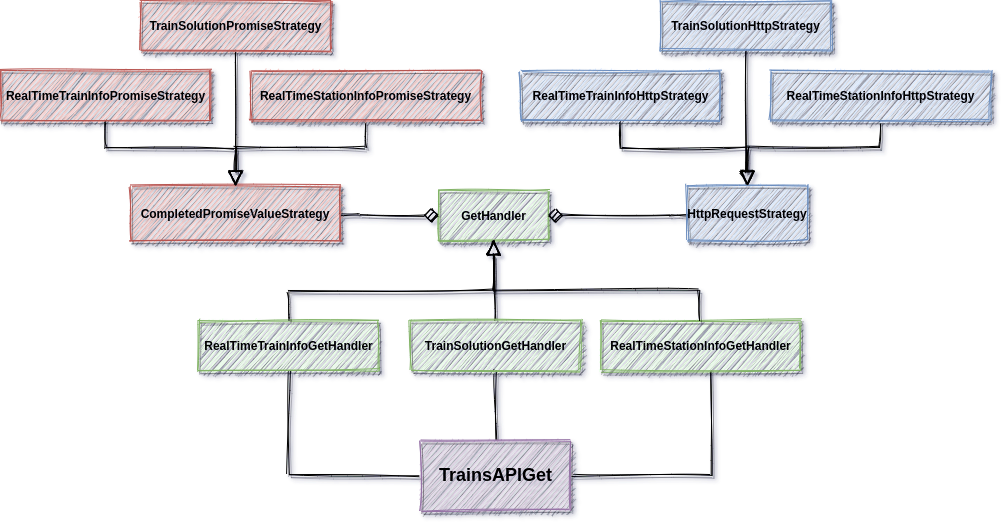
\includegraphics[width=160mm]{img/uml_2.png}
    \label{fig:uml_library}
\end{figure}

\begin{warn}[NOTA SUL DIAGRAMMA:]
Un generico GetHandler richiede una qualsiasi \textit{CompletedPromiseValueStrategy} ed una qualsiasi \textit{HttpRequestStrategy}.\newline L'implementazione \textit{TrainSolutionGetHandler} per esempio utilizza la classe implementata \textit{TrainSolutionPromiseStrategy} come \textit{CompletedPromiseValueStrategy} e  \textit{TrainSolutionHttpStrategy} come \textit{HttpRequestStrategy}.\newline Questi collegamenti sono stati omessi nel grafico per semplicità di illustrazione.\newline È implicito presupporre che le classi che implementano \textit{GetHandler} utilizzino strategy che hanno lo stesso nome.
\end{warn}

\subsubsection{Utilizzo della libreria}
Vert.X permette di creare un oggetto Router che fornisce metodi utili a creare nuove route. Tramite il metodo \textit{get()} si può creare una route che accetta richieste HTTP che utilizzano il metodo GET. Tramite il metodo \textit{handler()} è poi possibile associare un handler a partire dal context.
\begin{minted}{java}
    TrainsApiGET handlersGET = TrainsApiGET.createInstance(vertx);

    //adding to router GET routes and linking handlers from our API
    router.get("/train-solution")
          .handler(handlersGET::getTrainSolutions);
    //same as ctx -> handlersGET.getTrainSolutions(ctx)
    router.get("/real-time-train-info")
          .handler(handlersGET::getRealTimeTrainInfo);
    router.get("/real-time-station-info")
          .handler(handlersGET::getRealTimeStationInfo);
\end{minted}
